\documentclass[11pt,a4paper]{article}
\usepackage[T1]{fontenc}
\usepackage[utf8]{inputenc}
\usepackage[margin=19mm,headheight=14pt]{geometry}
\usepackage{lmodern,amsmath,amssymb,booktabs,xcolor,listings,enumitem,fancyhdr,graphicx}
\usepackage{placeins}
\usepackage[colorlinks=true,linkcolor=blue!50!black,urlcolor=blue!50!black]{hyperref}
\setlength{\parindent}{0pt}
\setlength{\parskip}{5pt}
\setlist[itemize]{leftmargin=*,topsep=3pt,itemsep=2pt,parsep=0pt}
\setlist[enumerate]{leftmargin=*,topsep=3pt,itemsep=2pt,parsep=0pt}
\pagestyle{fancy}
\fancyhf{}
\fancyhead[L]{Normalizing flows}
\fancyhead[R]{Teacher's guide}
\fancyfoot[C]{\thepage}
\definecolor{codebg}{RGB}{246,247,249}
\lstset{language=Python,basicstyle=\ttfamily\footnotesize,
  keywordstyle=\color{blue!55!black},commentstyle=\color{black!60},
  stringstyle=\color{green!35!black},backgroundcolor=\color{codebg},
  frame=single,rulecolor=\color{black!15},framesep=5pt,
  showstringspaces=false,keepspaces=true,columns=fullflexible,
  breaklines=true,aboveskip=6pt,belowskip=6pt}
\newcommand{\E}{\mathbb E}
\newcommand{\Var}{\operatorname{Var}}
\newcommand{\Cov}{\operatorname{Cov}}
\newcommand{\Normal}{\mathcal N}
\newcommand{\KL}{\operatorname{KL}}
\newcommand{\R}{\mathbb R}
\newcommand{\dd}{\,d}

% Keep all prose, titles, and section headings in normal weight.
\makeatletter
\renewcommand\section{\@startsection{section}{1}{\z@}%
  {-3.5ex \@plus -1ex \@minus -.2ex}%
  {2.3ex \@plus .2ex}{\normalfont\Large}}
\renewcommand\subsection{\@startsection{subsection}{2}{\z@}%
  {-3.25ex \@plus -1ex \@minus -.2ex}%
  {1.5ex \@plus .2ex}{\normalfont\large}}
\renewcommand\subsubsection{\@startsection{subsubsection}{3}{\z@}%
  {-3.25ex \@plus -1ex \@minus -.2ex}%
  {1.5ex \@plus .2ex}{\normalfont\normalsize}}
\makeatother
\begin{document}
\begin{center}
  {\LARGE Normalizing flows: from change of variables to learned densities}\\[6pt]
  {\large Teacher's guide and worked solutions}\\[3pt]
  Bayesian machine learning \textbar\ Skoltech
\end{center}

A normalizing flow transforms a simple random variable through an invertible
map. Its density follows from the change-of-variables formula. The seminar
builds this calculation from a scalar affine transformation, then uses affine
coupling layers and their compositions to learn a two-dimensional density.
Tasks 1--3 lead to a trained RealNVP model and a held-out comparison with a
fitted Gaussian. Task 4 extends the same ideas to GPU training on MNIST images,
including dequantization, image-space densities, and bits per dimension.
The optional Bayesian appendix uses the
same model family as a variational approximation to a curved, posterior-shaped
analytic benchmark. This benchmark is specified directly, rather than obtained
as the posterior of a fitted data model.

The main distinction to preserve throughout is between \emph{evaluating the
model density exactly} and \emph{representing the desired distribution exactly}.
The Jacobian formula gives the density of the chosen transformation, up to
ordinary floating-point error. It does not remove approximation, estimation,
or optimization error in learning that transformation.

The companion student and solutions notebooks have the same lesson order.
The student notebook contains four implementation tasks, supplied checks,
experiments, and interpretation questions. Tasks 1--3 form the 90-minute core;
Task 4 is a separate 45--60-minute GPU extension. The solutions notebook
contains the
worked code and executed figures. This guide adds board derivations, suggested
hints, answers to oral questions, and a route through the material in class.

\section{Teaching plan}
\subsection{The 90-minute lesson}
Exercise time is included in each block. This schedule covers Tasks 1--3 and
ends with a trained two-dimensional density model. Task 4 is a separate
45--60-minute GPU extension. Neither optional appendix is required for either
the core lesson or the image experiment.
\begin{center}
\begin{tabular}{@{}p{15mm}p{52mm}p{89mm}@{}}
\toprule
Clock & Topic & Student activity and intended result \\
\midrule
0--15 & Random variables, maps, and densities & Derive the volume correction;
fix the sampling and encoding directions. \\
15--25 & Task 1: scalar affine flow & Implement the transformation and density;
check the sign and the inverse. \\
25--40 & Affine coupling & Derive the inverse and triangular Jacobian;
explain why the neural network need not be invertible. \\
40--55 & Task 2: coupling layer & Implement both directions and per-sample
log determinants; inspect identity initialization and checks. \\
55--70 & Composition and Task 3 & {\raggedright Apply inverse layers in reverse order; implement
\texttt{log\_prob} and sampling.\par} \\
70--85 & Likelihood training and diagnostics & Run supplied training;
compare held-out log densities, samples, densities, and encoded observations. \\
85--90 & Wrap-up & Explain what is exact, what is learned, and how this
connects with sampling and the Laplace approximation. \\
\bottomrule
\end{tabular}
\end{center}

Before the seminar. Run the complete solutions notebook on the
classroom machine. The main lesson uses PyTorch, NumPy, Matplotlib, and the
notebook display tools; its two-dimensional data are generated locally.
Task 4 additionally needs TorchVision, a CUDA-capable GPU, and the MNIST
training and test files. Download and cache MNIST before class, confirm that
the installed PyTorch and TorchVision versions work together, and run the image
extension on the GPU in advance. Confirm that the core training experiment
completes on CPU and retain both sets of executed outputs. Use the
student notebook for projection and keep the solutions available separately.
Students need the chain rule, determinants, Gaussian densities, expectations,
and basic tensor operations. Review that a matrix multiplication and an
elementwise multiplication are different operations.

During the seminar. Follow the cells in order. Students write the
core mathematical implementations; data preparation, plotting, optimization,
and evaluation helpers are supplied. Ask pairs to switch the typing role
between tasks. A function that raises \texttt{NotImplementedError} is unfinished;
the notebook skips its dependent experiments. Other failures should remain
visible, because a shape error or a failed Jacobian check is useful evidence.

Protect the density-estimation endpoint. Start coupling by minute 25,
composition by minute 55, and the training comparison by minute 70. If an
implementation remains unfinished, show its missing mathematical step and
continue with the supplied working solution. Shorten neural-network mechanics
and plotting-code discussion before removing the inverse calculation or the
held-out comparison. Use saved outputs if runtime is longer on students'
machines. Do not add the variational appendix to the timed lesson by default.

\subsection{A 60-minute route}
Use minutes 0--10 for the change of variables and notation, 10--17 for Task 1,
17--27 for the coupling derivation, 27--37 for Task 2, 37--47 for composition
and Task 3, 47--57 for the supplied training results and diagnostics, and
57--60 for the closing questions. Show the automatic-differentiation Jacobian checks
without deriving their implementation. Reduce task coding to filling the
transformation and log-determinant expressions. Show an already executed
training run if necessary. Keep both directions, all three task contracts,
and the difference between exact density evaluation and a learned fit.

\subsection{A 45--60-minute GPU extension for Task 4}
Keep Task 4 outside the 90-minute core. Allocate 10--12 minutes to discrete
pixels, uniform dequantization, and the logit Jacobian; 10--15 minutes to the
image-likelihood implementation and checks; 15--20 minutes to the supplied
training and validation run; and 10--13 minutes to held-out bits per dimension,
independent samples, temperature changes, and latent interpolation. Run the
full training before class and retain its outputs. Use those outputs if the
classroom GPU cannot complete training within the allotted block; the teaching
time is not a hardware-independent runtime promise.

The image model and loop are supplied. Students implement the likelihood
plumbing in Task 4, where an omitted preprocessing Jacobian or a missing
$8$ in bits per dimension creates a measurable error. Explain the dequantization
bound before discussing image quality. Do not turn the extension into a
separate image-classification exercise: digit labels are not training targets.

\subsection{Board layout and notation}
Keep the convention below visible. Different references call different
directions ``forward''; identify the actual map before comparing formulas.
In this seminar \texttt{inverse=False} always means the generative direction.
\begin{center}
\begin{tabular}{@{}p{38mm}p{119mm}@{}}
\toprule
Symbol or object & Meaning \\
\midrule
$z\in\R^d$, $p_0$ & Base variable and its standard-normal density. \\
$x\in\R^d$, $q_\phi$ & Observation-space variable and the flow's density. \\
$x=g_\phi(z)$ & Generative map: easy base samples become model samples. \\
$z=f_\phi(x)=g_\phi^{-1}(x)$ & Encoding map used to evaluate the density at an observation. \\
$\log|\det Dh|$ & Log absolute determinant of the map actually applied, not
always of the generative map. \\
Batch arrays & Main examples have shape $(B,2)$; log densities and coupling
log determinants have shape $(B,)$. \\
$m\in\{0,1\}^d$ & Mask; a one identifies a coordinate preserved by a coupling layer. \\
\bottomrule
\end{tabular}
\end{center}

The essential board formula is
\[
\boxed{\quad
 \log q_\phi(x)
 =\log p_0(f_\phi(x))+\log|\det Df_\phi(x)|
 =\log p_0(z)-\log|\det Dg_\phi(z)|,
 \quad z=f_\phi(x).\quad}
\]
The two expressions use Jacobians of opposite directions, evaluated at
corresponding points. Their signs differ for that reason.

\section{Purpose and published applications: teacher background}
Use this section for preparation and optional discussion. In the timed core,
choose one application for a 60--90-second introduction, then return to the
change-of-variables derivation. The full set of examples is not an additional
block in the 90-minute schedule.

\subsection{The practical problem: a distribution that can be sampled and scored}
A useful probabilistic model often needs both operations. We want to draw
candidate images, physical configurations, or parameter values, and also to
evaluate the density assigned to each candidate. A flow learns coordinates
where a complicated distribution is related to a simple base. Its inverse
and Jacobian make the candidate's density available; its generative map makes
fresh candidates available. These operations support different applications,
but they do not determine the training objective by themselves.

Before showing an application, state the random variable, the information
available for training, and the quantity required at the end. The same
coupling architecture can serve three different statistical roles:
\begin{center}
\begin{tabular}{@{}p{34mm}p{57mm}p{66mm}@{}}
\toprule
Role & What is learned & What is supplied \\
\midrule
Density estimator & $q_\phi(x)$ for observations $x$ & Examples from the data
distribution; maximize their log densities. \\
Variational approximation & $q_\phi(\theta)$ for one target posterior & An
evaluable log posterior kernel; sample from the flow while optimizing an
ELBO or reverse-KL objective. \\
{\raggedright Conditional posterior estimator\par} & $q_\phi(\theta\mid d)$ across many datasets &
Simulated parameter--data pairs; fit a conditional density and then insert a
new observed dataset $d$. \\
\bottomrule
\end{tabular}
\end{center}
The first role appears in the moons and MNIST experiments. The second appears
in Appendix A. The third motivates the gravitational-wave example below.
None is automatically Bayesian inference over the network weights $\phi$.

\subsection{Scientific posterior inference: DINGO and gravitational waves}
Dax et al. use conditional normalizing flows in DINGO to approximate posterior
distributions of astrophysical source parameters given gravitational-wave
data. Training on simulated parameter--data pairs amortizes the cost across
future observations. Their DINGO-IS study analyzes 42 binary-black-hole events
from LIGO and Virgo and combines the fast learned posterior proposal with
likelihood-based importance sampling~\cite{dingo}.

This example needs both flow operations. It generates independent proposals
$\theta_i\sim q_\phi(\theta\mid d)$ and evaluates their proposal densities to
form weights
\[
 w_i=\frac{p(d\mid\theta_i)p(\theta_i)}{q_\phi(\theta_i\mid d)}.
\]
Weight concentration diagnoses the proposal's quality. Importance weighting
corrects expectation estimates under coverage and integrability assumptions;
it does not turn a finite collection into exact independent unweighted
posterior draws. Finite-sample and overlap limitations still matter. The
paper's application shows why a tractable learned density can be useful even
when an approximation needs external verification and correction.

For the board, contrast this with Appendix A. DINGO learns a conditional
posterior family from simulations across many datasets. Appendix A optimizes
one flow against one evaluable target kernel. Both return approximate
posterior distributions, but the source of training information and the
expectation defining the loss differ.

\subsection{Molecular equilibrium sampling: Boltzmann generators}
A molecular equilibrium target has the form
$\pi(x)\propto\exp[-\beta U(x)]$, where $x$ denotes a physical configuration
and $U$ its energy. Molecular dynamics and local Monte Carlo can spend long
periods within one metastable state. No\'e et al. introduce Boltzmann generators,
which learn invertible transformations for direct configuration proposals.
Their examples include a particle system and a conformational change of the
BPTI protein; they also study free-energy differences~\cite{boltzmann}.

The flow supplies configurations and a density. Its importance weights satisfy
\[
 w(x)\propto\frac{\exp[-\beta U(x)]}{q_\phi(x)},
\]
which makes reweighting and corrected sampling possible.
Energy-based training relates directly to the reverse-KL calculation in
Appendix A; example configurations can also help training. A low-energy,
visually plausible configuration is not an equilibrium probability estimate.
Correct observables depend on appropriate weights, support, and exploration
of relevant states. The purpose is to reduce the cost of obtaining useful
configurations, while retaining a way to assess and correct their probabilities.

\subsection{Image density estimation and generation}
RealNVP models images through invertible transformations with tractable
likelihoods~\cite{realnvp}. Flow++ improves image density estimation using
changes to dequantization and coupling design~\cite{flowpp}. These are concrete
uses of normalized density models, rather than classifiers that predict a
digit label. An image model assigns probability to pixel configurations and
can generate new configurations by transforming base draws.

Task 4 is a small teaching version of this use case. It makes the conversion
from integer pixels to a continuous density explicit and reports a held-out
coding-length bound in bits per dimension. It is not intended to reproduce
the scale or quality of the published image architectures. A useful
comparison controls the image representation and dequantization convention;
raw continuous log densities in different units are not directly comparable.

\subsection{What a likelihood cannot establish on its own}
High density is not the same statement as semantic familiarity or safety.
Nalisnick et al. demonstrate that image generative models, including flows,
can assign higher likelihood to an out-of-distribution image dataset than
to the dataset on which they were trained, including the CIFAR-10/SVHN
comparison~\cite{ood}. The exact density formula therefore does not by itself
provide a reliable out-of-distribution detector. Such a use requires a stated
detection rule and evaluation on relevant alternatives.

The corresponding lesson for all three applications is practical: exact
model scoring supports likelihood comparisons, weighting, and diagnostics.
It does not prove that a learned posterior is calibrated, a molecular sample
has an equilibrium law, or a generated image is representative of the data.
Ask students to identify the additional evidence needed in each example.

\section{From transformed samples to a density}
\subsection{Conservation of probability}
Let $Z$ have density $p_0$ and let $g:\R^d\to\R^d$ be a differentiable
bijection with differentiable inverse $f$ and nonzero Jacobian determinant.
Writing $X=g(Z)$ defines a distribution. To calculate its density, take a
small region around $z$. Locally, the map is approximately linear:
\[
 g(z+\delta)\approx g(z)+Dg(z)\delta.
\]
A linear map changes volume by its absolute determinant. Thus an infinitesimal
volume transforms as $\dd x=|\det Dg(z)|\dd z$. Probability mass is preserved:
\[
 q(x)\dd x=p_0(z)\dd z.
\]
Substitution gives
\[
 q(x)=\frac{p_0(z)}{|\det Dg(z)|}
     =p_0(f(x))|\det Df(x)|.
\]
The inverse function theorem gives
$Df(g(z))=[Dg(z)]^{-1}$, so the two forms agree. Taking logarithms produces
the board formula above. Smooth neural maps satisfy these conditions when
constructed as below; with piecewise differentiable networks, the corresponding
Jacobian formula applies almost everywhere.

The factor is an absolute determinant because volumes cannot be negative.
In one dimension, a decreasing transformation still has a valid positive
density. Our affine scales are positive exponentials, so their derivatives
are positive; this does not remove the absolute value from the general theorem.

\begin{figure}[htbp]
\centering
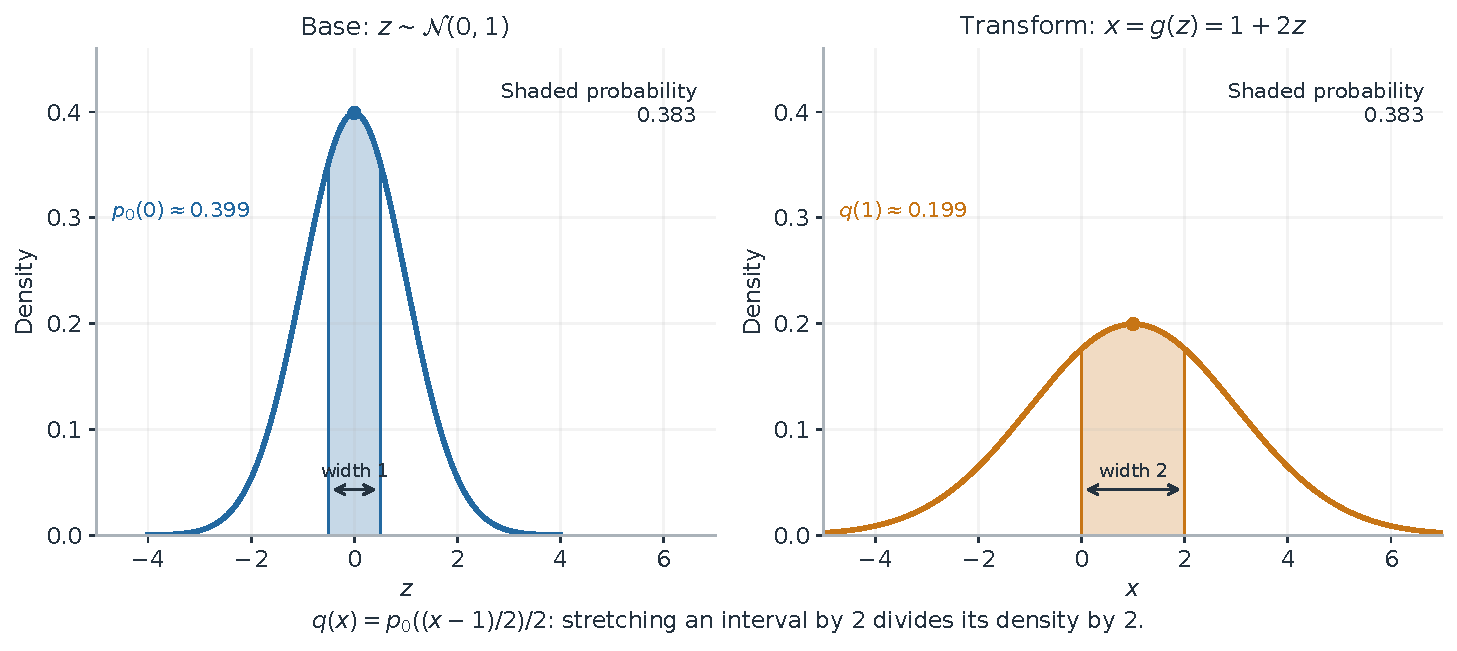
\includegraphics[width=0.98\linewidth]{assets/change_of_variables.pdf}
\caption{An invertible map transports probability mass and changes volume.
Expanding a region lowers its density per unit volume; contracting it raises
that density. The Jacobian determinant supplies the correction.}
\end{figure}

Oral prompt. If a transformation doubles the length of every small
interval, what happens to the density? It is divided by two at the corresponding
image points. Merely replacing $z$ by $f(x)$ in the base density does not account
for the change of units.

\subsection{Why the density is normalized}
Invertibility and a normalized base imply
\[
 \int_{\R^d}q(x)\dd x
 =\int_{\R^d}p_0(f(x))|\det Df(x)|\dd x
 =\int_{\R^d}p_0(z)\dd z=1.
\]
No partition function is estimated after training. This is a structural
property of the model family. It is separate from whether $q_\phi$ resembles
the distribution that generated the observations.

Ordinary sampling from a fitted flow requires independent base draws and one
application of $g_\phi$ to each draw. Conditional on the fitted parameters,
these are independent draws from $q_\phi$. They are draws from the desired
target only to the extent that $q_\phi$ equals that target. This separates a
flow sampler from an MCMC procedure designed to preserve a specified posterior.

\FloatBarrier
\section{Task 1: a scalar affine flow}
\subsection{What students should do}
Implement the two functions
\begin{lstlisting}
affine_1d(value, shift, log_scale, inverse=False)
affine_log_prob(x, shift, log_scale)
\end{lstlisting}
Both directions of the
transformation return the transformed tensor and the log absolute derivative
of the direction actually applied. For this scalar exercise, that second
output has the same shape as the input; it is not summed over a batch.
The shift and log scale may be Python scalars, so convert them to tensors with
the input's dtype and device before using tensor operations.

\subsection{Derivation and a numerical example}
Write $\mu$ for the shift and $a$ for the log scale:
\[
 x=g(z)=\mu+e^a z,\qquad
 z=f(x)=(x-\mu)e^{-a}.
\]
The forward derivative is $e^a$ and the inverse derivative is $e^{-a}$. Thus
\[
 \log|g'(z)|=a,\qquad \log|f'(x)|=-a.
\]
For $Z\sim\Normal(0,1)$,
\[
 \log q(x)=-\tfrac12z^2-\tfrac12\log(2\pi)-a,
 \qquad z=(x-\mu)e^{-a}.
\]
This is $\Normal(\mu,e^{2a})$: $e^a$ is the standard deviation, whereas
$e^{2a}$ is the variance. Parameterizing a positive scale by its logarithm
keeps it positive for every finite parameter value.

With $\mu=1$ and $a=\log2$, base points $(-1,0,1)$ become $(-1,1,3)$.
The forward log derivative is $\log2$, the inverse log derivative is
$-\log2$, and the density at the center is $1/(2\sqrt{2\pi})$. Its log density
is approximately $-1.61209$. The inverse recovers the original three points.

\subsection{Worked implementation}
\begin{lstlisting}
def affine_1d(value, shift, log_scale, inverse=False):
    shift = torch.as_tensor(shift, dtype=value.dtype, device=value.device)
    log_scale = torch.as_tensor(log_scale, dtype=value.dtype,
                                device=value.device)
    if inverse:
        transformed = (value - shift) * torch.exp(-log_scale)
        logdet = -log_scale
    else:
        transformed = shift + torch.exp(log_scale) * value
        logdet = log_scale
    return transformed, torch.ones_like(value) * logdet

def affine_log_prob(x, shift, log_scale):
    z, inverse_logdet = affine_1d(x, shift, log_scale,
                                 inverse=True)
    base_log_prob = -0.5 * (z.square() + math.log(2 * math.pi))
    return base_log_prob + inverse_logdet
\end{lstlisting}

\subsection{Checks, hints, and model answers}
The checks establish transformed values at two nonunit scales,
forward--inverse reconstruction, opposite log determinants at matching points,
and agreement with the analytic Gaussian density. Numerical integration of
the density checks normalization independently of reconstruction. An analytic
log-scale gradient is compared with automatic differentiation to verify that
tensor conversion and the inverse calculation preserve gradients. In the
executed reference run, 12,000 draws have sample mean 1.0021 and sample standard
deviation 2.0042, close to their analytic values 1 and 2.

A useful first hint is to write the inverse on paper. The second is to identify
which derivative each branch returns. For the density, evaluate the base at
the encoded point and \emph{add the inverse} log determinant. Do not subtract
it again.

Interpretation answer. Increasing $a$ stretches the distribution and
reduces its density at corresponding points by $e^{-a}$. It changes both the
encoded coordinate and the normalization term at a fixed $x$. Changing $\mu$
translates the distribution without changing the Jacobian. The determinant
correction is what makes the translated and scaled density integrate to one.

\section{Affine coupling: an invertible map from an ordinary network}
\subsection{A split into preserved and transformed coordinates}
Partition coordinates into $A$ and $B$. A coupling layer preserves $z_A$ and
uses a network evaluated at that preserved part to transform $z_B$:
\[
 x_A=z_A,\qquad
 x_B=z_B\odot\exp(s(z_A))+t(z_A).
\]
The operations on $B$ are elementwise. The functions $s$ and $t$ can be
ordinary neural networks; they need not be invertible. They produce
transformation parameters after the preserved coordinates are known.

The inverse is explicit:
\[
 z_A=x_A,\qquad
 z_B=(x_B-t(x_A))\odot\exp(-s(x_A)).
\]
The same network is evaluated at the same preserved values in both directions.
We solve the affine equation for the changed coordinates. We never solve for
the input of the neural network.

\subsection{The Jacobian and its determinant}
Order the coordinates as $(A,B)$. The generative Jacobian has block form
\[
 Dg(z)=\begin{pmatrix}
 I & 0\\
 * & \operatorname{diag}(e^{s(z_A)})
 \end{pmatrix}.
\]
The lower-left block includes derivatives of $s$ and $t$. It can be dense, but
it does not enter the determinant of this block-triangular matrix. Therefore
\[
 \det Dg(z)=\prod_{j\in B}e^{s_j(z_A)},\qquad
 \log|\det Dg(z)|=\sum_{j\in B}s_j(z_A).
\]
The inverse log determinant is the negative of the same sum. Translational
terms affect the map and its off-diagonal derivatives; they do not affect
this determinant. Autodifferentiation through the explicit inverse still
trains both networks through the full log density.

Board example. In two dimensions, preserve $z_1$ and write
$x_2=e^{s(z_1)}z_2+t(z_1)$. Its Jacobian is
\[
 \begin{pmatrix}
 1&0\\
 e^{s(z_1)}z_2s'(z_1)+t'(z_1)&e^{s(z_1)}
 \end{pmatrix}.
\]
The determinant is $e^{s(z_1)}$ even when the lower-left term is large.
The layer can bend a cloud through the dependence of the changed coordinate
on the preserved one, while retaining an inexpensive determinant.

\begin{figure}[htbp]
\centering
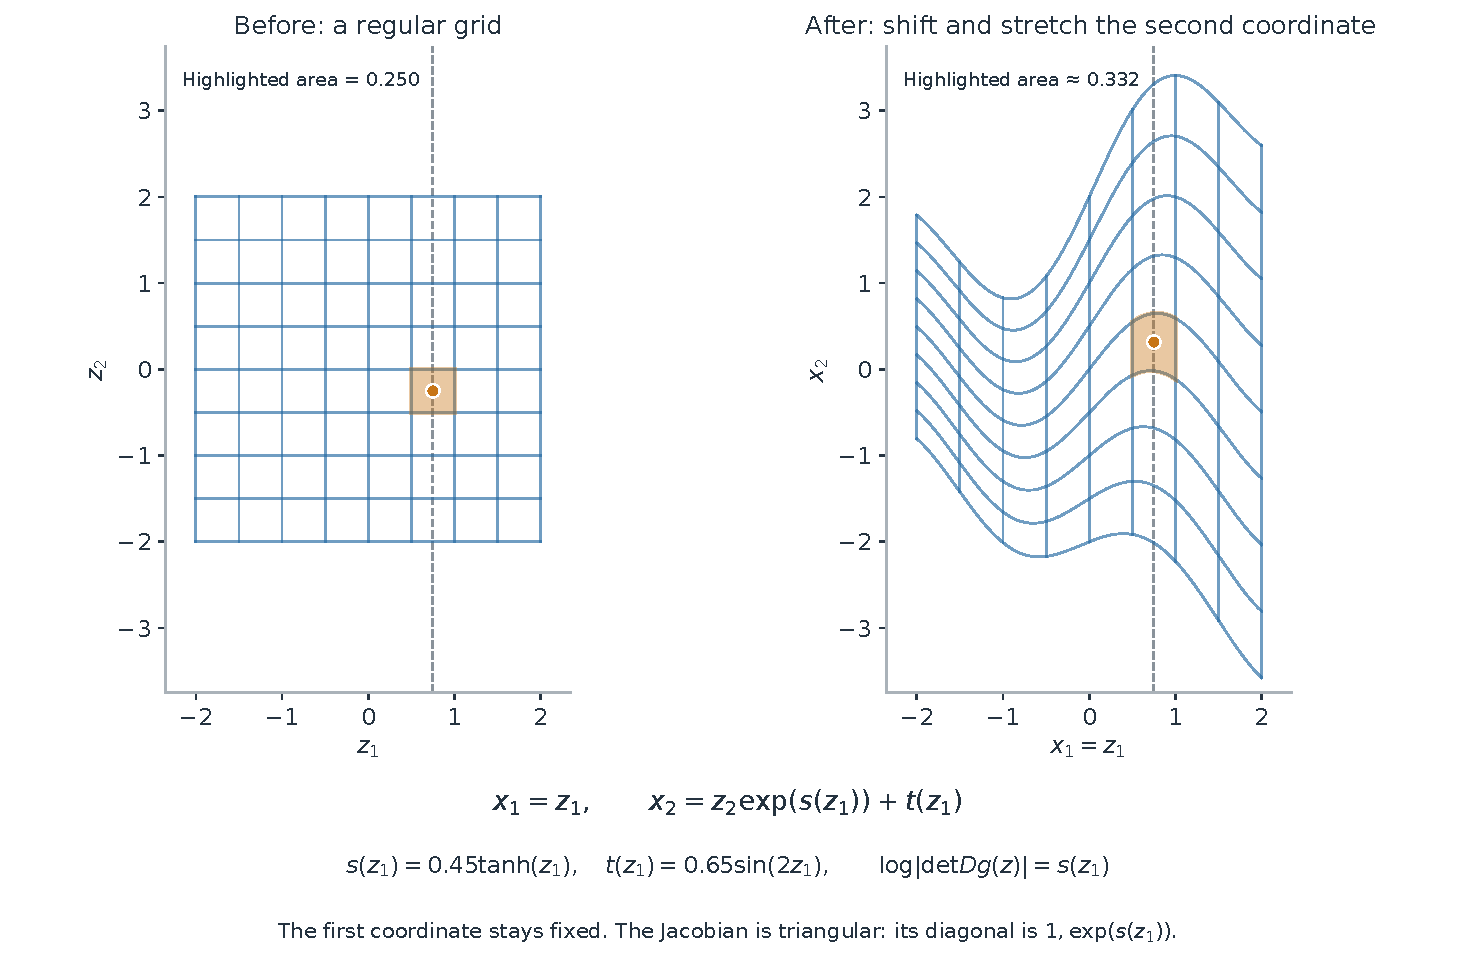
\includegraphics[width=0.98\linewidth]{assets/coupling_geometry.pdf}
\caption{A coupling layer preserves one coordinate and changes the other
through a scale and shift determined by the preserved coordinate. A nonlinear
shift can bend the sample cloud without requiring inversion of the network.}
\end{figure}

\subsection{Masks and bounded log scales}
The implementation keeps full-dimensional tensors and uses a binary mask $m$.
A one means ``preserve this coordinate''. Let
\[
 u=m\odot z,\qquad
 (s_{\rm raw},t_{\rm raw})=\operatorname{net}(u),
\]
where the network returns $2d$ entries split into two vectors of length $d$.
Set
\[
 s=1.5\tanh(s_{\rm raw})\odot(1-m),\qquad
 t=t_{\rm raw}\odot(1-m).
\]
Then
\[
 g(z)=m\odot z+(1-m)\odot(z\odot e^s+t).
\]
The network must receive the masked input. If its scale or shift depends on
a coordinate being transformed, this explicit inverse and triangular
Jacobian calculation no longer follow.

The bound limits each changed coordinate's log scale to $(-1.5,1.5)$.
Its scale is consequently between approximately $0.223$ and $4.482$.
This controls one source of numerical difficulty; it does not guarantee
stable gradients or a good fit for an arbitrary composition. The shift is not
bounded by this construction. Register the mask as a PyTorch buffer so it
moves with the module between devices and is saved with its state.

\FloatBarrier
\section{Task 2: implement a coupling layer}
\subsection{What students should do}
Complete the coupling layer's \texttt{transform} method. The argument
\texttt{inverse=False} selects generation; \texttt{inverse=True} selects
encoding. The supplied constructor stores the mask and network as
\texttt{self.mask} and \texttt{self.net}. It sets \texttt{scale\_limit} to 1.5.
The mask is a registered buffer. The final
network layer has zero weights and biases, so initially both scale and shift
are zero. This makes the whole coupling layer the identity without preventing
later optimization.

The derivation above allows general $d$; the supplied constructor implements
$d=2$ and accepts only masks $(1,0)$ and $(0,1)$. Its network has two hidden
layers of width 32 with hyperbolic-tangent activations and four output entries.
The method accepts a batch of shape $(B,2)$ and returns the transformed batch
and one log determinant per observation, of shape $(B,)$. Sum over coordinates
only. Return the determinant of the applied direction in both branches.

\subsection{Worked implementation}
\begin{lstlisting}
def transform(self, x, inverse=False):
    fixed = x * self.mask
    s_raw, t_raw = self.net(fixed).chunk(2, dim=-1)
    changed = 1.0 - self.mask
    s = self.scale_limit * torch.tanh(s_raw) * changed
    t = t_raw * changed
    if inverse:
        value = fixed + changed * (x - t) * torch.exp(-s)
        logdet = -s.sum(dim=-1)
    else:
        value = fixed + changed * (x * torch.exp(s) + t)
        logdet = s.sum(dim=-1)
    return value, logdet
\end{lstlisting}

In the inverse branch, \texttt{x} denotes the input to the encoding map,
which is the output of the generative map. Its preserved coordinates still
supply the same network inputs. A method's argument name need not encode the
mathematical direction; the \texttt{inverse} flag does.

\subsection{What the checks establish}
Identity initialization is useful but insufficient: an implementation that
always returns its input would pass that check. Nonzero final-layer parameters
are needed to test a genuine transformation. The supplied checks examine
preserved coordinates, forward--inverse reconstruction, cancellation of the
two log determinants at corresponding points, and agreement with an explicit
autodifferentiated Jacobian on a small two-dimensional example.

For a single input $z$, compare the reported forward log determinant with
\begin{lstlisting}
J = torch.autograd.functional.jacobian(
    lambda v: layer.transform(v[None, :])[0][0], z)
sign, reference_logdet = torch.linalg.slogdet(J)
\end{lstlisting}
Here the two-dimensional Jacobian is used only as a diagnostic. The normal
implementation uses the triangular formula rather than building a dense
Jacobian for every observation. Double precision makes this small comparison
more accurate. A forward--inverse check alone can miss a shared sign error
in two wrong log-determinant formulas.
The known linear conditioner also gives explicit expected coordinates and
determinants. This catches an implementation that consistently drops either
the shift or the scale, even if its own inverse and Jacobian still agree.

\subsection{Hints and interpretation answers}
Start by identifying the preserved coordinates, then evaluate the network once.
Mask its outputs before applying either branch. If reconstruction fails,
verify that the network receives the preserved part in both directions.
If reconstruction succeeds but densities disagree, inspect the determinant
sign and the axis of the sum.

Why not invert the neural network? Its inputs are copied unchanged
through the layer, so they are already available at the output. Once scale
and shift have been recomputed, each changed coordinate has a scalar affine
inverse.

Why are zero final-layer parameters acceptable? They initialize the
layer as the identity. During the first gradient update, the final layer can
receive nonzero gradients from its hidden features. Earlier layers may
initially receive zero gradient through zero final weights and begin changing
after the final weights move. Initializing every layer to zero would create a
different learning problem and is not required here.

Why not calculate a determinant numerically during training? A generic
dense determinant costs much more and hides the structural simplification.
The explicit small Jacobian is an independent check of the analytic expression.

\section{Composition: a RealNVP density model}
\subsection{Maps, inverses, and order}
Compose $K$ generative coupling layers:
\[
 h_0=z,\quad h_k=g_k(h_{k-1}),\quad
 x=h_K=g_K\circ\cdots\circ g_1(z).
\]
The chain rule and multiplicativity of determinants give
\[
 \log|\det Dg(z)|
 =\sum_{k=1}^K\log|\det Dg_k(h_{k-1})|.
\]
Encoding applies the last inverse first:
\[
 z=g_1^{-1}\circ\cdots\circ g_K^{-1}(x).
\]
When reading this composition right to left, the first operation on $x$ is
$g_K^{-1}$. In code, iterate through the layers in reverse order and pass
\texttt{inverse=True} to every layer. Their returned inverse log determinants
can simply be accumulated.

\begin{figure}[htbp]
\centering
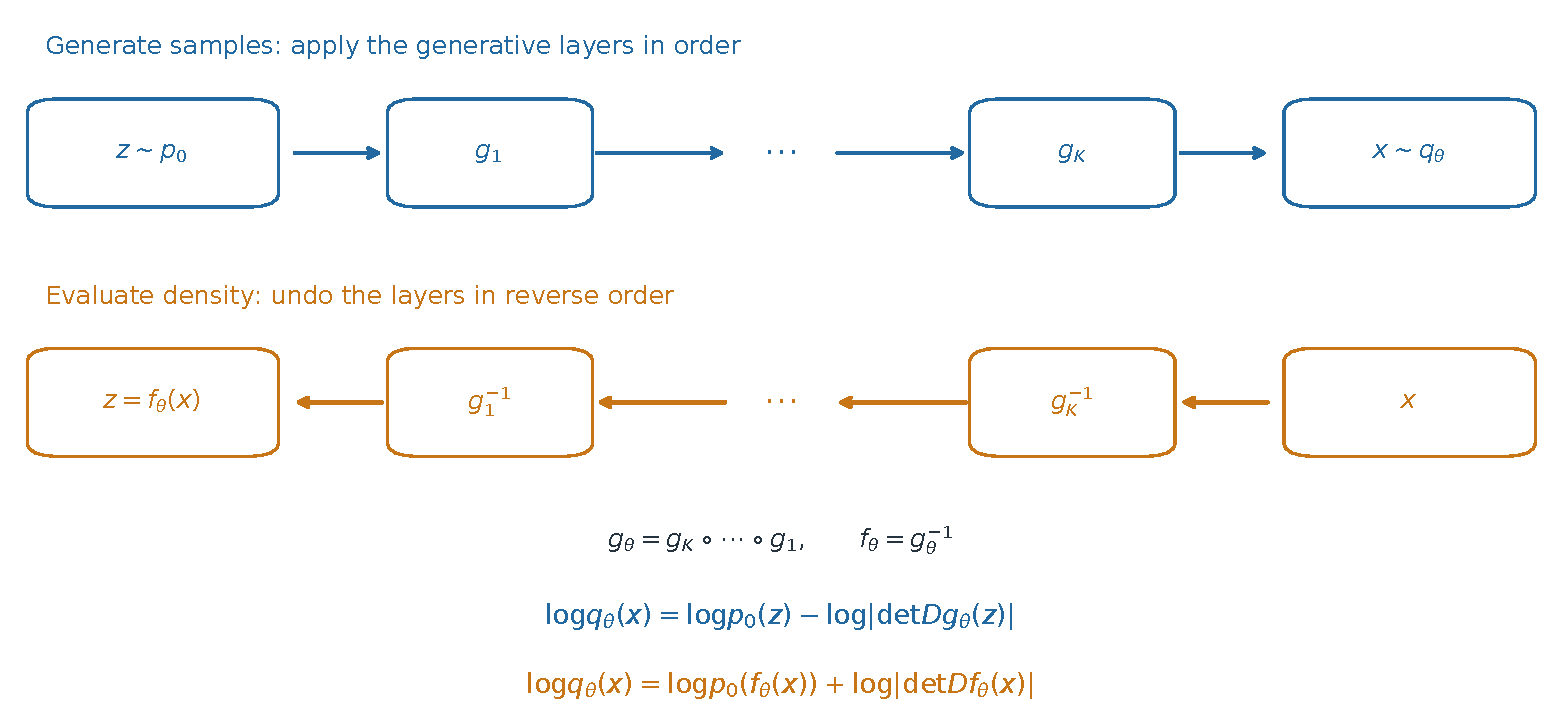
\includegraphics[width=0.98\linewidth]{assets/flow_directions.pdf}
\caption{Sampling follows the generative layers from the base to observations.
Density evaluation encodes an observation by applying inverse layers in reverse
order. Each layer reports the log determinant of the direction actually used.}
\end{figure}

\subsection{Why alternate masks?}
With mask $(1,0)$, the first coordinate is unchanged by a layer. If every layer
uses this same mask, the whole composition preserves the first coordinate,
so its marginal remains the base marginal. Nonlinear conditional changes in
the second coordinate cannot fix a wrong first-coordinate marginal.

The main model uses six layers with alternating masks $(1,0)$ and $(0,1)$.
Each coordinate can then be transformed using information carried by the
other coordinate. The default network has two hidden layers, each of width 32,
which keeps the toy problem inexpensive.
The number of layers and width are modeling choices; they do not establish
that every possible density is represented exactly.

\FloatBarrier
\section{Task 3: compose, score, and sample}
\subsection{What students should do}
Complete \texttt{RealNVP.transform}, \texttt{log\_prob}, and
\texttt{sample(n, generator=None)}.
The layers are stored in \texttt{self.layers}. The transformation returns
$(B,2)$ values and $(B,)$ log determinants. The supplied base-density
helper sums the coordinate log densities along the last axis. It returns
$(B,)$ values, not one number for the batch.

\subsection{Worked implementation}
\begin{lstlisting}
def transform(self, value, inverse=False):
    logdet = value.new_zeros(value.shape[0])
    layers = reversed(self.layers) if inverse else self.layers
    for layer in layers:
        value, contribution = layer.transform(value, inverse=inverse)
        logdet = logdet + contribution
    return value, logdet

def log_prob(self, x):
    z, inverse_logdet = self.transform(x, inverse=True)
    return standard_normal_log_prob(z) + inverse_logdet

@torch.no_grad()
def sample(self, n, generator=None):
    parameter = next(self.parameters())
    z = torch.randn(n, 2, generator=generator, dtype=parameter.dtype,
                    device=parameter.device)
    return self.transform(z, inverse=False)[0]
\end{lstlisting}

The optional random-number generator must match the model device. The
\texttt{sample} helper disables gradients for ordinary sampling. Training the
variational approximation instead uses \texttt{transform(z)} directly.

The standard-normal helper implements
\[
 \log p_0(z)=-\frac d2\log(2\pi)-\frac12\sum_{j=1}^d z_j^2.
\]
The inverse output already contains $\log|\det Df(x)|$. Add it when scoring
observations. If instead a sample has been generated and the forward
log determinant retained, the equivalent score is the base log density
\emph{minus} that forward log determinant.

\subsection{Checks and model answers}
The checks should include a nontrivial composition: all-identity layers cannot
expose a reversed-order error. Confirm reconstruction, opposite total log
determinants, score agreement along generated points, the sample shape, and
finite values. Gradients of the training objective must reach trainable
parameters. Do not put an encoding calculation inside \texttt{no\_grad} when
it is used for training; evaluation and plotting can use that context.
The supplied independent composition check uses
$g_1(z)=(z_1,2z_2+z_1)$ and $g_2(u)=(3u_1+u_2,u_2)$.
The expected output is $(4z_1+2z_2,z_1+2z_2)$ with log determinant $\log 6$.
This catches omitted layers and wrong order even when a round trip is
internally consistent.

Why must inverse layer order reverse? For two maps,
$g_2(g_1(z))=x$. Applying $g_2^{-1}$ first gives $g_1(z)$, and then applying
$g_1^{-1}$ gives $z$. Applying inverse maps in the original order generally
undoes neither composition.

Are model samples independent? Given fixed fitted parameters,
independent standard-normal base draws remain independent under the same
deterministic map. The transformed distribution is the learned $q_\phi$.
There is no accept/reject step or MCMC burn-in in ordinary flow sampling.

\section{Likelihood training on noisy two-moon observations}
\subsection{The objective and its statistical meaning}
The supplied data generator creates two semicircles with equal mixing
probabilities and adds independent Gaussian coordinate noise of standard
deviation 0.08. The labels color plots and are not training inputs. Generate
2,400 training, 600 validation, and 1,000 test observations with independent
random seeds. Optimize only with training observations:
\[
 \widehat L(\phi)=-\frac1{n_{\rm train}}
   \sum_{i=1}^{n_{\rm train}}\log q_\phi(x_i).
\]
The coordinate log densities and log determinants have already been summed
inside \texttt{log\_prob}. The final mean is over observations. PyTorch
backpropagates through the explicit inverse and the scale and shift networks;
Adam updates their parameters. The fixed main run uses six alternating
couplings with hidden width 32, 1,200 steps, minibatches of 256, and learning
rate $10^{-3}$. Gradient norms are clipped at 5. Full training and validation
NLL are evaluated every 100 steps; the best validation state is saved by deep
copy and restored before test evaluation. No determinant of a full
neural-network Jacobian is needed.

For a population density $p_{\rm data}$ and finite relevant expectations,
\[
 \KL(p_{\rm data}\Vert q_\phi)
 =\E_{p_{\rm data}}[\log p_{\rm data}(X)]
  -\E_{p_{\rm data}}[\log q_\phi(X)].
\]
The first term does not depend on $\phi$, so population maximum likelihood
minimizes this forward KL. The empirical loss estimates the cross-entropy
term from observations. A finite empirical distribution is a collection of
point masses; do not literally call its KL to a continuous density the
finite training loss.

\begin{lstlisting}
optimizer.zero_grad()
loss = -flow.log_prob(training_batch).mean()
loss.backward()
optimizer.step()
\end{lstlisting}

Initialization at the identity starts from the standard-normal density.
That is a diagnostic, not a fitted baseline. The Gaussian comparison is
fitted independently by maximum likelihood to the training set only.
For training observations $x_i$, its mean and covariance are
\[
 \widehat\mu=\frac1n\sum_i x_i,\qquad
 \widehat\Sigma=\frac1n\sum_i(x_i-\widehat\mu)(x_i-\widehat\mu)^\top.
\]
The MLE covariance uses $1/n$, not the unbiased $1/(n-1)$ factor. The supplied data have a nonsingular fitted covariance, so this baseline
does not add a diagonal regularizer. Fit no baseline parameters to validation
or test observations.

\subsection{Validation and held-out comparison}
The training budget and model size are fixed before test evaluation.
Validation observations select the checkpoint; the test set is evaluated after
that selection. The flow and Gaussian are scored on exactly the same held-out
observations in the same original units. The notebook reports negative log
likelihood (NLL), in nats per observation, so \emph{lower is better}.

The executed reference run restores step 1,200. Its results are:
\begin{center}
\begin{tabular}{@{}lrrrr@{}}
\toprule
Model & Train NLL & Validation NLL & Test NLL & Test SE \\
\midrule
Gaussian baseline & 1.9011 & 1.8794 & 1.9071 & 0.01779 \\
RealNVP & 0.9661 & 0.9069 & 0.9743 & 0.02312 \\
\bottomrule
\end{tabular}
\end{center}
The paired test loss difference, RealNVP minus Gaussian, is $-0.9328$ with
standard error $0.02768$. Its negative sign favors the flow. Use the paired
losses when discussing uncertainty of this comparison, because both fitted
models are evaluated on the same observations.

For pointwise losses $L_i=-\log q(x_i)$, the test standard error is
$s_L/\sqrt{n_{\rm test}}$. For a paired comparison, apply the same formula to
$D_i=L_i^{\rm flow}-L_i^{\rm Gaussian}$. These conditional standard errors
measure variation across new iid test samples with fitted models held fixed.
They do not include training randomness, checkpoint selection uncertainty,
or variation across new training/validation splits.

The lower flow NLL and its curved geometry favor the flexible model over a
single elliptical Gaussian on this problem. A better average score on one
finite test set does not certify every tail probability. The numerical values
above belong to the executed reference notebook; last digits can vary across
software versions. Do not require a universal training-loss threshold or
improvement at every optimization step.

If a flow does not outperform the Gaussian in a particular run, inspect the
mathematical checks and optimization history before interpreting the result.
A correctly evaluated flow density may still underfit, overfit, or be poorly
optimized. More training does not repair an incorrect inverse or determinant
sign.

\subsection{Read the diagnostic panels together}
\begin{enumerate}
\item Training and validation loss. Decreasing loss suggests the
optimizer is improving its objective. The plotted training and validation
losses are full-data averages evaluated under the same current parameters.
Their difference reflects different observations and fit, rather than a
comparison of differently timed minibatch values. A validation score slightly
better than the training score is possible with finite samples; it does not
by itself establish a data leak.
\item Density contours. A flow can place density along both curved
components. Plotting values on a finite grid does not integrate the full
model over $\R^2$. Visual gaps or small grid mass do not prove that the
density is unnormalized.
\item Generated samples. These show the learned distribution in
observation space. Compare geometry, component occupancy, and unusual points
with held-out observations. A pleasing scatterplot is not a likelihood check.
\item Encoded held-out observations. If $q_\phi=p_{\rm data}$, applying
$f_\phi$ to observations gives the base distribution. Approximately Gaussian
encoded data support the fit, but finite scatterplots and marginal histograms
can hide dependence and tail discrepancies. Encoding samples generated by the
same model gives the base by construction and principally checks the inverse.
\end{enumerate}

\subsection{Worked interpretation and closing prompts}
A suitable student explanation identifies the score direction, describes the
geometry that the flow learned, and gives a finite-data limitation. For example:
``The flow follows the curved components and has a lower held-out NLL in this
run. The negative paired loss difference favors the flow, and its standard
error measures new-test-sample variation at fixed fitted parameters. More
generated samples reduce integration error under the fitted density; they
do not change that density or repair a fitting error.''

The encoded test means in the reference run are approximately $(0.0048,-0.0349)$,
the marginal variances are $(0.922,1.042)$, and the covariance is $-0.0853$.
These are useful diagnostics, not exact moment identities for held-out data.
A mean near zero alone would not establish a correct joint distribution.

Connect with the preceding seminars. The Laplace approximation uses a
Gaussian derived from local posterior curvature. A flow provides a flexible
normalized family, but learning its parameters adds an optimization problem.
MCMC draws are dependent states designed to preserve a specified target;
ordinary fitted-flow draws are independent samples from a learned model.
A flow can also be used inside a corrected sampling method, but such a
correction is additional machinery and is outside this lesson.

Ask students to answer these three questions at the board:
\begin{enumerate}
\item Which direction evaluates the density at an observed $x$, and why?
\item Which mathematical property permits an ordinary neural network inside
an invertible coupling layer?
\item What remains approximate after a flow's Jacobian formula is implemented
correctly?
\end{enumerate}
The answers are encoding with the inverse, access to preserved coordinates
and a conditional affine inverse, and the learned approximation to the target
plus estimation and optimization error.

\section{Task 4: image density estimation on MNIST with a GPU}
\subsection{Purpose, scope, and preparation}
This is the 45--60-minute extension, rather than part of the 90-minute core.
It moves from two coordinates to all $28\times28=784$ image coordinates while
retaining the same generative convention. The supplied image model maps a
standard-normal base to logits, $y=g_\phi(z)$; the sigmoid then gives an image
in $(0,1)^{784}$. Density evaluation applies the inverse flow to the logits.
The objective fits pixel configurations, not digit labels. Labels appear only
in visualization captions.

The GPU experiment is enabled by \texttt{RUN\_MNIST = True}. Install a compatible
TorchVision alongside PyTorch and download MNIST before class. The default
cache is outside the seminar directory at \texttt{/tmp/sk\_bayes\_mnist}; set
\texttt{NF\_MNIST\_CACHE} before running the notebook to choose a persistent
location. A saved checkpoint is reused only when its recorded configuration
matches and checkpoint reuse is explicitly enabled. The default is
\texttt{MNIST\_RETRAIN = True}, which performs a fresh training run. Set it
to False for a cached demonstration. The CPU objective
and small-model checks run independently of CUDA availability. Without CUDA,
the training block prints an explicit skip message.

The image model, data preparation, optimizer, evaluation, and plots are
supplied. Students implement one function connecting integer pixels to the
flow's continuous density. Do not spend the exercise time reimplementing the
784-dimensional coupling constructor. Its mathematics is the same as Task 2,
with a larger mask and a different conditioner.

\subsection{Why integer pixels need dequantization}
An integer image is $I\in\{0,\ldots,255\}^D$, where $D=784$. A continuous
point has probability zero under a continuous density, so $q(I)$ is not the
probability of that integer image. Adding uniform noise lets a continuous
model represent probability mass within each integer-pixel bin. Draw
independent $\varepsilon_j\sim\operatorname{Uniform}(0,1)$ and set
\[
 u_j=\frac{I_j+\varepsilon_j}{256},\qquad
 y_j=\operatorname{logit}(u_j)=\log u_j-\log(1-u_j).
\]
The denominator is 256 because an 8-bit coordinate has 256 bins. Dividing by
255 here changes the bin width and can put bright pixels outside the intended
unit interval. The separate real-image display uses $I/255$ only to map display
intensities to the plotting range; it is not the density preprocessing.

The uncontracted logit is a bijection from $(0,1)^D$ to $\R^D$. Its derivative
is $1/[u_j(1-u_j)]$, so
\[
 \ell_{\rm pre}(u)
 :=\log\left|\det\frac{\partial y}{\partial u}\right|
 =\sum_{j=1}^D[-\log u_j-\log(1-u_j)].
\]
The flow's own density in logit coordinates is already provided by
\texttt{model.log\_prob(y)}. Converting it to normalized-pixel coordinates gives
\[
 \log q_u(u)=\log q_y(\operatorname{logit}(u))+\ell_{\rm pre}(u).
\]
These are two distinct corrections: the model includes its coupling and final
affine determinants; the task adds the logit determinant. Count each exactly
once.

The corresponding generative image map is
$u=\operatorname{sigmoid}(g_\phi(z))$. It maps the entire base space into the
open unit cube, and the resulting $q_u$ integrates to one there. The experiment
does not contract the unit interval, clip likelihood inputs, or use clipped
values to define a different density.

\subsection{From a continuous density to discrete likelihood and bits}
The normalized discrete model assigns an image the probability of its bin:
\begin{align*}
 P_\phi(I)
 &=\int_{\prod_j[I_j/256,(I_j+1)/256)}q_u(u)\dd u\\
 &=\int_{[0,1)^D}\frac{q_u((I+\varepsilon)/256)}{256^D}\dd\varepsilon.
\end{align*}
The 256 bins partition the unit interval, so summing these masses over all
integer images gives one. Jensen's inequality yields
\[
 \log P_\phi(I)
 \geq\E_\varepsilon[\log q_u((I+\varepsilon)/256)]-D\log256.
\]
This is the uniform-dequantization likelihood bound discussed in the flow
literature~\cite{realnvp,flowpp}. The exercise returns the random loss
\begin{align*}
 L(I,\varepsilon)
 &=-\log q_y(y)-\ell_{\rm pre}(u)+D\log256,\\
 \operatorname{bpd}(I,\varepsilon)
 &=\frac{L(I,\varepsilon)}{D\log2}
 =8-\frac{\log q_u(u)}{D\log2}.
\end{align*}
Here \texttt{nll\_nats} means $L$, including the discrete-bin correction.
Its noise expectation is an upper bound on the exact discrete NLL. One
individual noise realization is a Monte Carlo estimate of that bound and need
not itself upper-bound the exact NLL. Report the held-out average as a
dequantized bits-per-dimension score, not an exact discrete pixel likelihood.
Lower bpd is better under the same image representation and convention.

The logit preprocessing is fixed with respect to the learned parameters.
Consequently its Jacobian term and the bin correction do not change gradients
in $\phi$ when the same logits are used. They are essential to the score's
meaning and units. A decreasing training curve can therefore coexist with
incorrect reported bpd if either term is omitted. The flow's own determinant,
in contrast, generally depends on $\phi$ and is part of its learning signal.

\subsection{Implementation contract and worked answer}
Implement the function
\begin{lstlisting}
mnist_nll_terms(model, images, noise)
\end{lstlisting}
The input \texttt{images} has dtype uint8 and shape $(B,1,28,28)$.
The supplied noise has the same shape and values strictly between zero and
one. Return \texttt{nll\_nats} and \texttt{bits\_per\_dim}, each of shape $(B,)$.
The supplied preprocessing performs the logit calculation in float64. Cast
its outputs to the model's dtype and device without disabling gradients
through the model.

\begin{lstlisting}
def mnist_nll_terms(model, images, noise):
    parameter = next(model.parameters())
    y, preprocessing_logdet = mnist_preprocess(images, noise)
    y = y.to(device=parameter.device, dtype=parameter.dtype)
    preprocessing_logdet = preprocessing_logdet.to(
        device=parameter.device, dtype=parameter.dtype)
    log_density_u = model.log_prob(y) + preprocessing_logdet
    nll_nats = -log_density_u + MNIST_DIM * math.log(256)
    return nll_nats, nll_nats / (MNIST_DIM * math.log(2))
\end{lstlisting}

A useful first hint is to write the two density spaces, $q_y$ and $q_u$, on
paper. Next identify the Jacobian of the map actually applied during scoring.
Finally convert nats per image to bits per pixel. The optimizer takes the
mean of the returned bpd across the batch; the helper must not reduce the
batch dimension itself.

Numerical endpoints matter. With a bright pixel, float32 can round
$(I+\varepsilon)/256$ to one before the logarithm. The supplied helper uses
float64 noise and preprocessing, redraws exact zero noise values, and then
casts the logits to model precision. Replacing the preprocessing with
\texttt{images.float()/255} or clipping the logits changes the specified
calculation. The density checks use both zero-valued and 255-valued pixels.

\subsection{Independent checks before training}
The uniform-pixel oracle has logit density
\[
 q_y(y)=\prod_{j=1}^D\operatorname{sigmoid}(y_j)
                        [1-\operatorname{sigmoid}(y_j)].
\]
Its implied pixel density is $q_u(u)=1$: the logit density and preprocessing
Jacobian cancel. Therefore every integer image has bin probability $256^{-D}$,
$L=D\log256$, and bpd exactly 8, for every supplied noise draw. This checks
normalization units and the Jacobian sign without relying on the image flow.
The second oracle uses independent normal logits and compares the result
with a separately written scalar expression. A parameter-gradient check
ensures that the task has not detached the model density.

The supplied image model also has a small CPU check with nonzero coupling
parameters and a nontrivial final affine map. It verifies reconstruction,
determinant cancellation, and density agreement. Passing these checks permits
training; a favorable training result does not replace them.

\subsection{The supplied image flow and training-only initialization}
The default model has 14,691,168 trainable parameters and ten affine coupling
layers. Each preserves half of a
flattened $28\times28$ checkerboard and transforms the other half; masks
alternate. Each conditioner is an MLP with two width-512 hidden layers and
SiLU activations. Its final linear layer starts at zero. Changed-coordinate
log scales use $1.5\tanh(s_{\rm raw})$, as in the core lesson.

A final generative affine map gives every pixel its own logit location and
scale:
\[
 y=\mu+\exp(a)\odot h,\qquad
 \log|\det Dy/Dh|=\sum_{j=1}^D a_j.
\]
Both \texttt{location} and \texttt{log\_scale} are trainable parameters.
Initialize them from the mean and standard deviation of dequantized logits
for the first 8,192 training-split images, flooring initialization standard
deviations at 0.1 before taking logarithms. This gives useful starting
coordinates. No validation or test image supplies initialization moments.
During encoding, undo this affine map before the reversed coupling layers;
its inverse log determinant is $-\sum_j a_j$.

This MLP is an educational likelihood model. It does not implement the
convolutional and multiscale image architecture of the original RealNVP paper.
The 784-dimensional model is supplied so students can concentrate on the
change of variables and the statistical interpretation of its score.

\subsection{Data separation, checkpointing, and runtime}
Shuffle the official 60,000-image MNIST training set once with a fixed seed.
Use 50,000 images to fit the model and 10,000 for validation. Keep the official
10,000-image test set for evaluation after selecting and restoring the best
validation checkpoint. Labels never enter the likelihood or parameter updates.

Train for twelve epochs with batch size 256, Adam starting at learning rate
$5\times10^{-4}$, cosine scheduling to $5\times10^{-5}$, and gradient-norm
clipping at 5. Use fresh independent dequantization noise for each training
batch. Validation and test images have fixed independent noise draws, so
checkpoint comparisons and repeated evaluation use the same points. All
settings are chosen before examining test results.

The plotted training curve averages minibatch losses collected while the
parameters change during an epoch. Validation uses one fixed checkpoint and
fixed noise. These curves consequently have different averaging conventions,
whereas the core moons curves evaluate full training and validation losses
under the same checkpoint. Discuss the overall trend and selected epoch
without requiring the curves to coincide or decrease monotonically.

\subsection{Reference results from the executed GPU run}
The complete reference notebook ran the actual twelve-epoch training loop on
an NVIDIA L40. Training took about 53 seconds in this run; this is an observed
runtime for that hardware and software stack, not a promise for other GPUs.
Validation selected epoch 12. The initial validation score was 2.6201 bpd;
the final results were:
\begin{center}
\begin{tabular}{@{}lr@{}}
\toprule
Quantity & Dequantized bits per dimension \\
\midrule
Epoch-12 training average, online/fresh noise & 1.7810 \\
Selected validation score, fixed noise & 1.7909 \\
Held-out test mean, fixed noise & 1.7844 \\
Test standard error across image/noise pairs & 0.0030011 \\
\bottomrule
\end{tabular}
\end{center}
The test result is an evaluation of the selected model, not a criterion used
to choose its training duration. Values in another software stack can differ.
A cached demonstration reports the original training duration; checkpoint
loading is a separate action. Keep the executed outputs available for slower
classroom hardware.

\subsection{Read scores, generated images, and transformations separately}
The test table reports mean dequantized bpd and its standard error across
held-out image/noise pairs, conditional on the fitted model. This estimates
variation across new pairs under the same scoring scheme. It omits randomness
from fitting, initialization and split selection, approximation error, and
the gap between the dequantization bound and exact discrete NLL.

The notebook compares consecutive held-out observations with unfiltered
independent model draws at temperature one. It does not use class conditioning
or discard unattractive generations. Incomplete or ambiguous digits reveal
limitations that an average score may conceal. An unconditional density model
is not a digit classifier, and image quality is not a classification accuracy.

\begin{figure}[htbp]
\centering
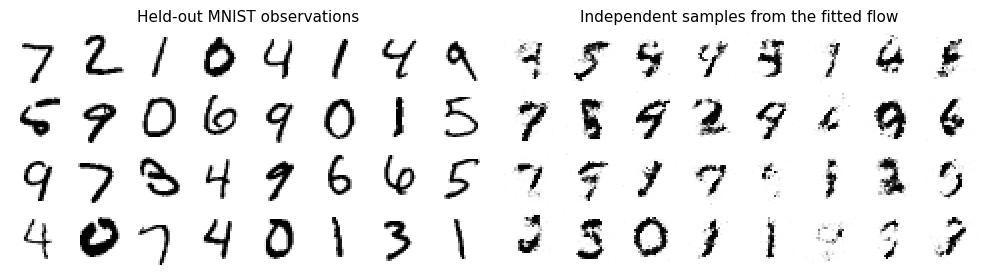
\includegraphics[width=\linewidth]{assets/mnist_samples.pdf}
\caption{Actual reference-run output. Left: 32 consecutive held-out MNIST
images. Right: 32 unfiltered independent draws at temperature one from the
fitted flow, with the same grayscale limits. Several samples have recognizable
digit shapes, while incomplete strokes and extra marks show remaining
modeling limitations. These are generated configurations, not predicted labels.}
\end{figure}

The temperature panels use the same base draws at $T=0.65$, $0.85$, and $1$.
Replacing $z$ with $Tz$ changes the base to $\Normal(0,T^2I)$ and hence changes
the generated distribution. Only $T=1$ samples the model whose score was
reported. Cleaner-looking examples at a lower temperature do not improve the
likelihood or establish a better fit for the original model.

For latent interpolation, encode consecutive held-out image pairs, linearly
interpolate their latent vectors, and decode the path. The digit labels only
caption its endpoints. These paths are deterministic, not independent
samples. A line between typical high-dimensional Gaussian points can pass
through atypical latent regions; a smooth visual transition does not prove
that the learned density is correct.

Finally, encode a dequantized held-out image and decode that same latent
vector. Near-perfect reconstruction checks numerical invertibility, which
holds structurally even for a poorly fitted flow. The displayed error map has
a magnified color scale; do not interpret it as generation quality. The
diagnostic uses an independent float64 copy of the fitted model and retains
the original float64 dequantized logits and pixels. It checks maximum pixel
error below $2\times10^{-10}$, logit reconstruction with absolute and relative
tolerances $10^{-9}$, and determinant cancellation with absolute tolerance
$10^{-8}$. Training and reported scores still use float32. The higher-precision
copy reduces numerical roundoff for this separate check; it does not refit
the model or improve its learned distribution.
The reference maximum errors are $1.55\times10^{-15}$ in pixel values,
$7.11\times10^{-15}$ in logits, and $1.14\times10^{-13}$ for determinant
cancellation. These are numerical inversion results, not measures of the
flow's approximation error.

\FloatBarrier
\subsection{Worked interpretation and teaching prompts}
A suitable explanation identifies both coordinate systems and the discrete
bin correction, then separates evaluation from visualization. For example:
``The logit determinant converts a density per unit logit to one per unit
normalized pixel. The $784\log256$ term accounts for the integer bins. The
reported bpd is a dequantization-bound estimate, while independent images
show which configurations the fitted model produces. Reconstruction checks
an inverse and does not guarantee that fresh model samples look like digits.''

Ask students which terms affect parameter gradients, which change reported
units, and which operations change the sampled distribution. Then ask them
to explain why setting a lower temperature, collecting more model samples,
and taking more optimizer steps address three different aspects of the result.

\section{Debugging reference}
\begin{center}
\begin{tabular}{@{}p{44mm}p{113mm}@{}}
\toprule
Observed problem & Check first \\
\midrule
Inverse fails after one layer & The network sees only preserved coordinates;
the inverse subtracts the shift before multiplying by the inverse scale. \\
{\raggedright Inverse fails only after composition\par} & Reverse the layer order as well as
the direction of each layer. \\
Inverse works, density fails & Check determinant direction, its sign, and
whether the determinant belongs to the actually applied map. \\
{\raggedright One scalar log determinant for a batch\par} & Sum on the coordinate axis
\texttt{dim=-1}; retain one value per observation. \\
No learned change in one coordinate & Inspect masks; identical masks preserve
one marginal through the entire composition. \\
Only identity tests pass & Test after assigning nonzero final-layer parameters;
identity initialization hides several implementation errors. \\
Non-finite loss or gradients & Inspect scale bounds, learning rate, data scale,
and the first layer producing non-finite values. Do not silently clip log
probabilities to make a failed check pass. \\
Parameters never change & Verify an optimizer step follows backward,
gradients are enabled, and the intended parameters are registered. \\
CPU/device mismatch & Register masks as buffers; create scalar constants and
base samples with matching dtype and device. \\
Attractive samples, poor test score & Check train-only preprocessing and
baseline fitting, inverse scoring, model capacity, and train/validation fit. \\
MNIST score off by 8 bpd & Include $784\log256$ inside the returned NLL
before dividing by $784\log2$. \\
Non-finite MNIST logits & Preserve float64 dequantization preprocessing,
strictly interior noise, and the divisor 256. \\
{\raggedright MNIST inverse succeeds but samples look poor\par} & Reconstruction tests the
invertible architecture; independent generations assess the fitted density. \\
Unexpected cached image model & Check the configuration and the explicit
\texttt{MNIST\_RETRAIN} setting before interpreting a new run. \\
\bottomrule
\end{tabular}
\end{center}

\appendix
\section{A flow as a Bayesian variational approximation}
This appendix is optional and fully supplied; it introduces no additional
implementation task beyond Tasks 1--4. After completing Tasks 2 and 3, enable it in setup:
\begin{lstlisting}
RUN_APPENDICES = True
\end{lstlisting}
It reuses the flow and optimizer to approximate a curved,
posterior-shaped analytic benchmark, keeping the density calculation separate
from the choice of training objective. The target is specified directly and
is not the posterior of a fitted data model. Its exact transport, moments,
and direct draws provide checks without relying on another approximate
inference method.

\subsection{A curved, normalized banana target}
Let
\[
 \Theta_1=Z_1,\qquad
 \Theta_2=b(Z_1^2-1)+\sigma Z_2,\qquad
 (Z_1,Z_2)\sim\Normal(0,I_2),
\]
with $b=0.8$ and $\sigma=0.45$. Equivalently,
\[
 \pi(\theta)=\Normal(\theta_1;0,1)\,
         \Normal(\theta_2;b(\theta_1^2-1),\sigma^2).
\]
The exact transport is invertible, with
$z_1=\theta_1$, $z_2=[\theta_2-b(\theta_1^2-1)]/\sigma$ and constant generative determinant
$\sigma$. Its log density is
\[
 \log\pi(\theta)=-\log(2\pi)-\log\sigma
 -\tfrac12\theta_1^2
 -\frac{[\theta_2-b(\theta_1^2-1)]^2}{2\sigma^2}.
\]
Conditional integration over $\theta_2$ followed by integration over $\theta_1$ shows
normalization immediately. The shape is curved, despite both base variables
and the conditional observation noise being Gaussian.

\subsection{Exact moments and a local Laplace comparison}
For a standard-normal variable,
$\E Z_1^2=1$, $\E Z_1^3=0$, and $\E Z_1^4=3$. Thus
\begin{align*}
 \E \Theta_1&=0,& \E \Theta_2&=b(\E Z_1^2-1)=0,\\
 \Var \Theta_1&=1,&
 \Var \Theta_2&=b^2\Var(Z_1^2)+\sigma^2=2b^2+\sigma^2,\\
 \Cov(\Theta_1,\Theta_2)&=b\E[Z_1(Z_1^2-1)]=0.
\end{align*}
Consequently
\[
 \E_\pi\Theta=(0,0)^\top,\qquad
 \Cov_\pi\Theta=\operatorname{diag}(1,1.4825).
\]
Zero covariance does not imply independence: the conditional mean of $\Theta_2$
depends on $\Theta_1^2$.

Write $r=\theta_2-b(\theta_1^2-1)$. Apart from a constant, the negative log density is
\[
 J(\theta)=\tfrac12\theta_1^2+\frac{r^2}{2\sigma^2}.
\]
It is minimized uniquely at $\theta_{\rm MAP}=(0,-b)=(0,-0.8)$, where $r=0$.
At that point $\nabla r=(0,1)^\top$, so
\[
 \nabla^2J(\theta_{\rm MAP})
 =\begin{pmatrix}1&0\\0&\sigma^{-2}\end{pmatrix},\qquad
 q_{\rm L}=\Normal\!\left(
 \begin{pmatrix}0\\-0.8\end{pmatrix},
 \begin{pmatrix}1&0\\0&0.2025\end{pmatrix}\right).
\]
The exact target mean is not its mode. The local Gaussian misses the vertical
variation induced by the curved conditional mean. This makes a direct link
to the preceding Laplace seminar: positive local curvature yields a valid
Gaussian approximation, without guaranteeing global moment accuracy.

\subsection{Reverse-KL training}
Suppose the target is given by an evaluable kernel $\widetilde\pi$ with
normalizer $Z$. A variational objective is
\[
 \KL(q_\phi\Vert\pi)
 =\E_{q_\phi}[\log q_\phi(\Theta)-\log\widetilde\pi(\Theta)]+\log Z.
\]
The unknown $\log Z$ is constant in $\phi$, so it can be omitted while
optimizing. Generate $\Theta=g_\phi(Z_0)$ using $Z_0\sim p_0$. The
reparameterized objective is
\[
 L_{\rm VI}(\phi)=\E_{Z_0\sim p_0}\left[
 \log p_0(Z_0)-\log|\det Dg_\phi(Z_0)|
 -\log\widetilde\pi(g_\phi(Z_0))\right].
\]
The supplied run uses a fresh six-layer, width-32 model, Adam with
learning rate $10^{-3}$, 1,400 steps, base minibatches of 512, and gradient-norm
clipping at 5. Fresh base draws give a stochastic estimate. Backpropagate through the
transformed samples, the forward log determinant, and the target evaluation.
Do not detach the samples. The base density term is constant with respect
to $\phi$ for a fixed base sample, but retaining it permits an interpretable
Monte Carlo objective value.

\begin{lstlisting}
z = torch.randn(batch_size, 2, device=DEVICE, dtype=DTYPE)
theta, forward_logdet = flow.transform(z)
log_q = standard_normal_log_prob(z) - forward_logdet
loss = (log_q - banana_log_prob(theta)).mean()
optimizer.zero_grad()
loss.backward()
optimizer.step()
\end{lstlisting}
For the fully normalized banana density, this loss estimates
$\KL(q_\phi\Vert\pi)$. If the target function omits a log normalizing
constant, it estimates that KL minus $\log Z$, so its numerical value is
not itself a KL. Even an estimate of the normalized KL can be slightly negative
because a finite Monte Carlo estimate fluctuates; the exact KL is nonnegative.

\subsection{How to assess the variational approximation}
Compare 20,000 independent samples from each of the trained flow, the exact
transport, and the Laplace Gaussian, using new random seeds after training.
The supplied table reports means, the second marginal variance,
$\Pr(\Theta_2>1)$ with its event Monte Carlo standard error, and reverse KL
with its integrand Monte Carlo standard error. Do not reuse the last
optimization minibatch as an evaluation sample.

The banana's moments above are analytic references. A tail probability estimated
from a large exact-transport sample still has Monte Carlo error. Conditional
integration also gives the deterministic one-dimensional reference
\[
 \Pr_\pi(\Theta_2>c)=
 \int_{-\infty}^{\infty}\varphi(u)
 \left[1-\Phi\left(\frac{c-b(u^2-1)}\sigma\right)\right]\dd u,
\]
where $\varphi$ and $\Phi$ are the standard-normal density and CDF. This integral
can be evaluated by numerical quadrature. In the supplied notebook,
320-node Gauss--Hermite quadrature gives $\Pr_\pi(\Theta_2>1)\simeq0.14437009$;
256 nodes give 0.14437012. Their agreement is a useful numerical check, rather
than an analytic expression for this probability. State whether a reported
reference is analytic, quadrature-based, or sampled.

As an optional algebraic audit, the Laplace approximation in this particular
example has
\[
 \KL(q_{\rm L}\Vert\pi)
 =\KL(\pi\Vert q_{\rm L})
 =\frac{3b^2}{2\sigma^2}\simeq4.74074.
\]
For the reverse direction, write $\Theta_1=Z_1$ and $\Theta_2=-b+\sigma Z_2$ under
$q_{\rm L}$. Then the target residual is $\sigma Z_2-bZ_1^2$, whose squared
expectation is $\sigma^2+3b^2$. The log normalizing constants and the first
coordinate terms cancel. The forward direction has the same value because
under the target $\Theta_2+b=bZ_1^2+\sigma Z_2$. Equality of these two KL values
is a property of this example, not a general symmetry of KL divergence.

\subsection{Reference numerical results and interpretation}
The executed run gives the following illustrative evaluation values:
\begin{center}
\begin{tabular}{@{}lrrrr@{}}
\toprule
Distribution & Mean 2 & Variance 2 & $\Pr(\Theta_2>1)$ & Reverse-KL estimate \\
\midrule
Exact target draws & 0.0107 & 1.5204 & 0.14665 & 0 \\
Laplace draws & $-0.7961$ & 0.2019 & 0 observed & 4.5788 \\
Variational flow & $-0.0662$ & 1.1533 & 0.13595 & 0.01934 \\
\bottomrule
\end{tabular}
\end{center}
The flow KL estimate has Monte Carlo standard error $0.00192$, and its event
estimate has standard error $0.00242$. The target-reference event estimate
has standard error $0.00250$. The flow follows the curved mass much better
than Laplace, but its second-coordinate variance is still below the analytic
value 1.4825. The flow event estimate 0.13595 is also below the quadrature
reference 0.14437. Present this remaining error rather than calling the learned
target exact or its moments fully recovered.

The Laplace event requires special care. Analytically,
\[
 \Pr_{q_{\rm L}}(\Theta_2>1)
 =1-\Phi\!\left(\frac{1+b}{\sigma}\right)
 =1-\Phi(4)\simeq3.1671\times10^{-5}.
\]
With 20,000 draws the expected event count is only 0.6334. Zero observed
events, and hence a zero plug-in Bernoulli standard error in the displayed
table, are quite plausible. Neither implies that the event probability or
its estimation uncertainty is zero. The Laplace KL estimate 4.5788 has
Monte Carlo standard error 0.1042; compare it with the analytic value 4.7407,
allowing for sampling variation.

Interpretation answer. The target mean averages the entire curved
mass and need not equal the density mode. The trained flow improves the
geometry and many summaries relative to Laplace, while retaining visible
approximation error. Its model density is exactly evaluable even when its
moments or tails disagree with the target. More draws reduce numerical error
under the fitted flow; they do not eliminate this discrepancy. With an unknown
target normalizer, the same VI gradients remain available, but the absolute
KL value cannot be recovered from the kernel objective alone. Exact target
moments and independent reference draws would usually be unavailable too.

\section{Support, expressiveness, and the direction of KL}
\subsection{Support constraints}
A finite composition of the stated coupling bijections maps $\R^d$ onto
$\R^d$. With a positive standard-normal base, the model density is positive
throughout this space. It cannot assign exactly zero density to an open gap
or produce a distribution exactly supported on a lower-dimensional curve.
Noisy moons provide an ordinary continuous example; an ideal noiseless
one-dimensional curve in $\R^2$ has no two-dimensional Lebesgue density.

A connected full-support model can nevertheless place very little probability
between separated high-density regions and can represent multiple density
modes. ``A bijection cannot produce a multimodal density from a Gaussian'' is
false: the spatially varying Jacobian changes density heights. What remains
constrained here is the exact support, as well as the finite model's capacity.
Targets restricted to a positive domain or a simplex require an appropriate
additional support transformation and its Jacobian.

\subsection{Computational and modeling tradeoffs}
The coupling structure makes both the inverse and determinant inexpensive.
A single layer leaves some coordinates unchanged, so composition and changed
masks are essential. Additional layers and network width increase flexibility
and computational cost. Bounded scales help numerics while also restricting
what a fixed number of layers can express. None of these choices removes the
need for held-out evaluation or a target-specific adequacy check.

Density values depend on units: rescaling coordinates changes a log density
by the corresponding log-Jacobian term. Compare models on the same transformed
data, or consistently convert all scores back to original units. Differential
log densities can be positive, and a negative average negative log likelihood
is not by itself an error.

\subsection{Likelihood and variational objectives ask different questions}
\begin{center}
\begin{tabular}{@{}p{32mm}p{60mm}p{65mm}@{}}
\toprule
Training setting & Objective and source of samples & Main implication \\
\midrule
Density estimation & $-\E_{p_{\rm data}}\log q_\phi$;
samples come from observations. & {\raggedright Population objective differs from
$\KL(p_{\rm data}\Vert q_\phi)$ by a constant.\par} \\
{\raggedright Variational inference\par} & $\E_{q_\phi}[\log q_\phi-\log\widetilde\pi]$;
samples come from the flow. & Objective differs from
$\KL(q_\phi\Vert\pi)$ by a constant independent of $\phi$. \\
\bottomrule
\end{tabular}
\end{center}

Forward KL penalizes assigning too little density where the target supplies
probability mass. Reverse KL averages over where the current approximation
places its own mass; missed regions may contribute little to its sampled
objective. These observations explain familiar tendencies, but do not justify
blanket promises that likelihood covers every mode or reverse KL always
selects one mode. Model family, support, target geometry, data coverage, and
optimization all matter. For an exactly representable target, a global
minimum of either KL is obtained at $q_\phi=\pi$ when the divergences are
well-defined.

Final oral prompt. Can more samples from a fitted flow repair a wrong
variational approximation? More samples reduce Monte Carlo error for
expectations under that fitted $q_\phi$, under the usual moment assumptions.
They do not change $q_\phi$ or eliminate its discrepancy from the target.
That is the same distinction between numerical uncertainty and inferential
approximation emphasized in the sampling and Laplace seminars.

\begin{thebibliography}{9}
\bibitem{realnvp}
Laurent Dinh, Jascha Sohl-Dickstein, and Samy Bengio.
\emph{Density estimation using Real NVP}. ICLR, 2017.
\href{https://arxiv.org/abs/1605.08803}{arXiv:1605.08803}.

\bibitem{rezende}
Danilo Jimenez Rezende and Shakir Mohamed.
\emph{Variational inference with normalizing flows}. ICML, 2015.
\href{https://arxiv.org/abs/1505.05770}{arXiv:1505.05770}.

\bibitem{dingo}
Maximilian Dax, Stephen R. Green, Jonathan Gair, Michael P\"urrer,
Jonas Wildberger, Jakob H. Macke, Alessandra Buonanno, and Bernhard Sch\"olkopf.
\emph{Neural importance sampling for rapid and reliable gravitational-wave inference}.
Physical Review Letters, 130:171403, 2023.
\href{https://arxiv.org/abs/2210.05686}{arXiv:2210.05686};
\href{https://doi.org/10.1103/PhysRevLett.130.171403}{published article}.

\bibitem{boltzmann}
Frank No\'e, Simon Olsson, Jonas K\"ohler, and Hao Wu.
\emph{Boltzmann generators: sampling equilibrium states of many-body systems
with deep learning}. Science, 365:eaaw1147, 2019.
\href{https://arxiv.org/abs/1812.01729}{arXiv:1812.01729};
\href{https://doi.org/10.1126/science.aaw1147}{published article}.

\bibitem{flowpp}
Jonathan Ho, Xi Chen, Aravind Srinivas, Yan Duan, and Pieter Abbeel.
\emph{Flow++: improving flow-based generative models with variational
dequantization and architecture design}. ICML, 2019.
\href{https://proceedings.mlr.press/v97/ho19a.html}{PMLR 97:2722--2730}.

\bibitem{ood}
Eric Nalisnick, Akihiro Matsukawa, Yee Whye Teh, Dilan Gorur, and
Balaji Lakshminarayanan.
\emph{Do deep generative models know what they don't know?} ICLR, 2019.
\href{https://arxiv.org/abs/1810.09136}{arXiv:1810.09136}.
\end{thebibliography}
\end{document}
